% ****************************************************************************************
% ************************      REPORTE DE BASE DE DATOS     *****************************
% ****************************************************************************************

%  =======================================================
% =======         HEADER FOR DOCUMENT        ============
% =======================================================
    % *********   DOCUMENT ITSELF   **************
    \documentclass[12pt, fleqn]{article}                             %Type of docuemtn and size of font and left eq
    \usepackage[margin=1.2in]{geometry}                             %Margins and Geometry pacakge
    \usepackage{ifthen}                                             %Allow simple programming
    \usepackage{hyperref}                                           %Create MetaData for a PDF and LINKS!
    \hypersetup{pageanchor=false}                                   %Solve 'double page 1' warnings in build
    \setlength{\parindent}{0pt}                                     %Eliminate ugly indentation
    \author{Oscar Andrés Rosas}                                     %Who I am

    % *********   LANGUAJE AND UFT-8   *********
    \usepackage[spanish]{babel}                                     %Please use spanish
    \usepackage[utf8]{inputenc}                                     %Please use spanish - UFT
    \usepackage[T1]{fontenc}                                        %Please use spanish
    \usepackage{textcmds}                                           %Allow us to use quoutes
    \usepackage{changepage}                                         %Allow us to use identate paragraphs
    \usepackage{lipsum}                                             %Allow to put dummy text

    % *********   MATH AND HIS STYLE  *********
    \usepackage{ntheorem, amsmath, amssymb, amsfonts}               %All fucking math, I want all!
    \usepackage{mathrsfs, mathtools, empheq}                        %All fucking math, I want all!
    \usepackage{centernot}                                          %Allow me to negate a symbol
    \decimalpoint                                                   %Use decimal point

    % *********   GRAPHICS AND IMAGES *********
    \usepackage{graphicx}                                           %Allow to create graphics
    \usepackage{wrapfig}                                            %Allow to create images
    \graphicspath{ {Graphics/} }                                    %Where are the images :D

    % *********   LISTS AND TABLES ***********
    \usepackage{listings}                                           %We will be using code here
    \usepackage[inline]{enumitem}                                   %We will need to enumarate
    \usepackage{tasks}                                              %Horizontal lists
    \usepackage{longtable}                                          %Lets make tables awesome
    \usepackage{booktabs}                                           %Lets make tables awesome
    \usepackage{tabularx}                                           %Lets make tables awesome
    \usepackage{multirow}                                           %Lets make tables awesome
    \usepackage{multicol}                                           %Create multicolumns

    % *********   HEADERS AND FOOTERS ********
    \usepackage{fancyhdr}                                           %Lets make awesome headers/footers
    \pagestyle{fancy}                                               %Lets make awesome headers/footers
    \setlength{\headheight}{16pt}                                   %Top line
    \setlength{\parskip}{0.5em}                                     %Top line
    \renewcommand{\footrulewidth}{0.5pt}                            %Bottom line

    \lhead{                                                         %Left Header
        \hyperlink{section.\arabic{section}}                        %Make a link to the current chapter
        {\normalsize{\textsc{\nouppercase{\leftmark}}}}             %And fot it put the name
    }

    \rhead{                                                         %Right Header
        \hyperlink{section.\arabic{section}.\arabic{subsection}}    %Make a link to the current chapter
            {\footnotesize{\textsc{\nouppercase{\rightmark}}}}      %And fot it put the name
    }

    \rfoot{\textsc{\small{Practica 5}}}                             %This will always be a footer  

    \fancyfoot[L]{                                                  %Algoritm for a changing footer
        \ifthenelse{\isodd{\value{page}}}                           %IF ODD PAGE:
            {\href{https://compilandoconocimiento.com/yo/}          %DO THIS:
                {\footnotesize                                      %Send the page
                    {\textsc{Oscar Andrés Rosas}}}}                 %Send the page
            {\href{https://compilandoconocimiento.com}              %ELSE DO THIS: 
                {\footnotesize                                      %Send the author
                    {\textsc{Compilando Conocimiento}}}}            %Send the author
    }
    
    
    
  
% ========================================
% ===========   COMMANDS    ==============
% ========================================

    % =====  GENERAL TEXT  ==========
    \newcommand \Quote {\qq}                                        %Use: \Quote to use quotes
    \newcommand \Over {\overline}                                   %Use: \Bar to use just for short
    \newcommand \ForceNewLine {$\Space$\\}                          %Use it in theorems for example
    
    \newenvironment{Indentation}[1][0.75em]                         %Use: \begin{Inde...}[Num]...\end{Inde...}
    {\begin{adjustwidth}{#1}{}}                                     %If you dont put nothing i will use 0.75 em
    {\end{adjustwidth}}                                             %This indentate a paragraph
    \newenvironment{SmallIndentation}[1][0.75em]                    %Use: The same that we upper one, just 
    {\begin{adjustwidth}{#1}{}\begin{footnotesize}}                 %footnotesize size of letter by default
    {\end{footnotesize}\end{adjustwidth}}                           %that's it


    % =====  GENERAL MATH  ==========
    \DeclareMathOperator \Space {\quad}                             %Use: \Space for a cool mega space
    \DeclareMathOperator \MiniSpace {\;}                            %Use: \Space for a cool mini space
    \newcommand \Such {\MiniSpace|\MiniSpace}                       %Use: \Such like in sets
    \newcommand \Also {\MiniSpace \text{y} \MiniSpace}              %Use: \Also so it's look cool
    \newcommand \Remember[1]{\Space\text{\scriptsize{#1}}}          %Use: \Remember so it's look cool

    \newtheorem{Theorem}{Teorema}[section]                          %Use: \begin{Theorem}[Name]\label{Nombre}...
    \newtheorem{Corollary}{Colorario}[Theorem]                      %Use: \begin{Corollary}[Name]\label{Nombre}...
    \newtheorem{Lemma}[Theorem]{Lemma}                              %Use: \begin{Lemma}[Name]\label{Nombre}...
    \newtheorem{Definition}{Definición}[section]                    %Use: \begin{Definition}[Name]\label{Nombre}...

    \newcommand{\Set}[1]{\left\{ \MiniSpace #1 \MiniSpace \right\}} %Use: \Set {Info}
    \newcommand{\Brackets}[1]{\left[ #1 \right]}                    %Use: \Brackets {Info} 
    \newcommand{\Wrap}[1]{\left( #1 \right)}                        %Use: \Wrap {Info} 
    \newcommand{\pfrac}[2]{\Wrap{\dfrac{#1}{#2}}}                   %Use: Put fractions in parentesis

    \newenvironment{MultiLineEquation}[1]                           %Use: To create MultiLine equations
        {\begin{equation}\begin{alignedat}{#1}}                     %Use: \begin{Multi..}{Num. de Columnas}
        {\end{alignedat}\end{equation}}                             %And.. that's it!
    \newenvironment{MultiLineEquation*}[1]                          %Use: To create MultiLine equations
        {\begin{equation*}\begin{alignedat}{#1}}                    %Use: \begin{Multi..}{Num. de Columnas}
        {\end{alignedat}\end{equation*}}                            %And.. that's it!


    % =====  LOGIC  ==================
    \DeclareMathOperator \doublearrow {\leftrightarrow}             %Use: \doublearrow for a double arrow
    \newcommand \lequal {\MiniSpace \Leftrightarrow \MiniSpace}     %Use: \lequal for a double arrow
    \newcommand \linfire {\MiniSpace \Rightarrow \MiniSpace}        %Use: \lequal for a double arrow
    \newcommand \longto {\longrightarrow}                           %Use: \longto for a long arrow

    % =====  NUMBER THEORY  ==========
    \DeclareMathOperator \Naturals  {\mathbb{N}}                     %Use: \Naturals por Notation
    \DeclareMathOperator \Primes    {\mathbb{P}}                     %Use: \Naturals por Notation
    \DeclareMathOperator \Integers  {\mathbb{Z}}                     %Use: \Integers por Notation
    \DeclareMathOperator \Racionals {\mathbb{Q}}                     %Use: \Racionals por Notation
    \DeclareMathOperator \Reals     {\mathbb{R}}                     %Use: \Reals por Notation
    \DeclareMathOperator \Complexs  {\mathbb{C}}                     %Use: \Complex por Notation

    % === LINEAL ALGEBRA & VECTORS ===
    \DeclareMathOperator \LinealTransformation {\mathcal{T}}        %Use: \LinealTransformation for a cool T
    \newcommand{\Mag}[1]{\left| #1 \right|}                         %Use: \Mag {Info} 

    \newcommand{\pVector}[1]{                                       %Use: \pVector {Matrix Notation} use parentesis
        \ensuremath{\begin{pmatrix}#1\end{pmatrix}}                 %Example: \pVector{a\\b\\c} or \pVector{a&b&c} 
    }
    \newcommand{\lVector}[1]{                                       %Use: \lVector {Matrix Notation} use a abs 
        \ensuremath{\begin{vmatrix}#1\end{vmatrix}}                 %Example: \lVector{a\\b\\c} or \lVector{a&b&c} 
    }
    \newcommand{\bVector}[1]{                                       %Use: \bVector {Matrix Notation} use a brackets 
        \ensuremath{\begin{bmatrix}#1\end{bmatrix}}                 %Example: \bVector{a\\b\\c} or \bVector{a&b&c} 
    }
    \newcommand{\Vector}[1]{                                        %Use: \Vector {Matrix Notation} no parentesis
        \ensuremath{\begin{matrix}#1\end{matrix}}                   %Example: \Vector{a\\b\\c} or \Vector{a&b&c}
    }

    % MATRIX
    \makeatletter                                                   %Example: \begin{matrix}[cc|c]
    \renewcommand*\env@matrix[1][*\c@MaxMatrixCols c] {             %WTF! IS THIS
        \hskip -\arraycolsep                                        %WTF! IS THIS
        \let\@ifnextchar\new@ifnextchar                             %WTF! IS THIS
        \array{#1}                                                  %WTF! IS THIS
    }                                                               %WTF! IS THIS
    \makeatother                                                    %WTF! IS THIS

    % TRIGONOMETRIC FUNCTIONS
    \newcommand{\Cos}[1]{\cos\Wrap{#1}}                             %Simple wrappers
    \newcommand{\Sin}[1]{\sin\Wrap{#1}}                             %Simple wrappers

    % === COMPLEX ANALYSIS ===
    \newcommand \Cis[1]  {\Cos{#1} + i \Sin{#1}}                    %Use: \Cis for cos(x) + i sin(x)
    \newcommand \pCis[1] {\Wrap{\Cis{#1}}}                          %Use: \pCis for the same ut parantesis
    \newcommand \bCis[1] {\Brackets{\Cis{#1}}}                      %Use: \bCis for the same to Brackets

    % === CALCULUS ===
    \newcommand \Partial[2] {\dfrac{\partial #1}{\partial #2}}      %Use: \Partial for simple use

    % =====  GENERAL COLOR  =========
    \definecolor{IndigoMD}{HTML}{3F51B5}                            %Use: Color :D
    \definecolor{DeepPurpleMD}{HTML}{673AB7}                        %Use: Color :D
    \definecolor{TealMD}{HTML}{009688}                              %Use: Color :D        
    \definecolor{BlueGrey800MD}{HTML}{37474F}                       %Use: Color :D
    \definecolor{BlueGrey100MD}{HTML}{CFD8DC}                       %Use: Color :D
    \definecolor{IndigoMD}{HTML}{3F51B5}                            %Use: Color :D
    \definecolor{Green100MD}{HTML}{DCEDC8}                          %Use: Color :D

    \newenvironment{ColorText}[1]{                                  %Use: \begin{ColorText}
        \leavevmode\color{#1}\ignorespaces}                         %That's is!


    % =====  CODE EDITOR =========
    \lstdefinestyle{CompilandoStyle} {                              %This is Code Style
        backgroundcolor=\color{BlueGrey800MD},                      %Background Color  
        basicstyle=\tiny\color{white},                              %Font color
        commentstyle=\color{BlueGrey100MD},                         %Comment color
        stringstyle=\color{TealMD},                                 %String color
        keywordstyle=\color{Green100MD},                            %keywords color
        numberstyle=\tiny\color{TealMD},                            %Size of a number
        frame=shadowbox,                                            %Adds a frame around the code
        breakatwhitespace=true,                                     %Style                       
        breaklines=true,                                            %Style                   
        keepspaces=true,                                            %Style                   
        numbers=left,                                               %Style                   
        numbersep=10pt,                                             %Style 
        xleftmargin=\parindent,                                     %Style 
        tabsize=4                                                   %Style 
    }
 
    \lstset{style=CompilandoStyle}                                  %Use this style



% =====================================================
% ============        COVER PAGE       ================
% =====================================================
\begin{document}
\begin{titlepage}

    \center
    % ============ UNIVERSITY NAME AND DATA =========
    \textsc{\Large ESCOM - IPN}\\[0.5cm] 
    \textsc{\large Bases de Datos 2CM12}\\[1.5cm]

    % ============ NAME OF THE DOCUMENT  ============
    \rule{\linewidth}{0.5mm} \\[1.0cm]
        { \huge \bfseries Vistas}\\[1.0cm] 
    \rule{\linewidth}{0.5mm} \\[2.0cm]
     
    % ============  MY INFORMATION  =================
    \begin{minipage}{0.4\textwidth}
        \begin{flushleft} \large
            \textbf{\textsc{Alumno:}}\\
            Rosas Hernandez Oscar Andres
        \end{flushleft}
    \end{minipage}
    ~
    \begin{minipage}{0.4\textwidth}
        \begin{flushright} \large
            \textbf{\textsc{Profesor: }}\\
            Euler Hernandez Contreras
        \end{flushright}
    \end{minipage}\\[3,5cm]

    % ====== SEMI TITLE ==========
    {\LARGE Reporte 5}\\[4cm] 
    
    
    \vfill

\end{titlepage}









% ===============================================================================
% ===================        QUERIES EN SQL                ======================
% ===============================================================================
\section{Views en SQL}


    En teoría de bases de datos, una vista es una consulta que se presenta como una tabla (virtual)
    a partir de un conjunto de tablas en una base de datos relacional.

    Las vistas tienen la misma estructura que una tabla: filas y columnas.
    La única diferencia es que sólo \textbf{se almacena de ellas la definición, no los datos}.
    Los cambios aplicados a los datos en una tabla se reflejan en los datos mostrados en invocaciones
    posteriores de la vista.
    En algunas bases de datos NoSQL, las vistas son la única forma de consultar datos.

    Los datos que se recuperan mediante una consulta a una vista se presentarán igual que los de una tabla.

    Una vista se crea a través de una expresión de consulta (una sentencia SELECT) que la calcula y que puede
    realizarse sobre una o más tablas.


    % ========================================
    % =========     VENTAJAS     =============
    % ========================================
    \subsection{Ventajas}

        Las vistas pueden ofrecer ventajas sobre las tablas:

        \begin{itemize}

            \item
                Las vistas pueden representar un subconjunto de los datos contenidos en una tabla.
                En consecuencia, una vista puede limitar el grado de exposición a las tablas al mundo exterior:
                un usuario dado puede tener permiso para consultar la vista, mientras que se deniega el acceso
                al resto de la tabla base.

            \item
                Las vistas pueden ocultar la complejidad de los datos.
                Por ejemplo, una vista podría aparecer como Sales2000 o Sales2001, particionando
                de forma transparente la tabla subyacente real.

            \item 
                Las vistas cuestan muy poco espacio para almacenar; la base de datos contiene sólo
                la definición de una vista, no una copia de todos los datos que presenta.

        \end{itemize}



    % ========================================
    % =========    SINTAXIS      =============
    % ========================================
    \subsection{Sintaxis}

        Empecemos por la sentencia general de las vistas:

        \begin{lstlisting}[language=SQL, gobble=12]
            CREATE VIEW ViewName AS
                SELECT FielName
                    FROM TableName
                    WHERE Conditions
                    ORDER BY FielName; 
        \end{lstlisting}

       

% ===============================================================================
% ===================             PRACTICA 3               ======================
% ===============================================================================
\clearpage
\section{Parte Practica: Practica 3}

    Veamor por pasos que es lo que hicimos:

    \begin{itemize}

        \item
            \textbf{Mostramos: Nombre de la Sucursal y el estado donde esta}
            \lstinputlisting[language=SQL, linerange={6-10}]{Practica5.sql}

        \item
            \textbf{Mostramos: Nombre del Producto y su Categoria}
            \lstinputlisting[language=SQL, linerange={14-21}]{Practica5.sql}

        \item
            \textbf{Mostramos: Nombre de la Categoria y Subcategoria}
            \lstinputlisting[language=SQL, linerange={25-31}]{Practica5.sql}

        \item
            \textbf{Mostramos: Nombre del Cliente y Sucursal donde fue dado de alta}
            \lstinputlisting[language=SQL, linerange={35-46}]{Practica5.sql}

        \item
            \textbf{Mostramos: Nombre del Producto y su Subcategoria}
            \lstinputlisting[language=SQL, linerange={50-58}]{Practica5.sql}


        \item
            \textbf{Mostramos: Nombre del Cliente y monto del Credito}
            \lstinputlisting[language=SQL, linerange={62-73}]{Practica5.sql}

        \item
            \textbf{Mostramos: Nombre del Cliente y fechas de pago}
            \lstinputlisting[language=SQL, linerange={75-85}]{Practica5.sql}

        \item
            \textbf{Mostramos: Nombre del Producto y Precio Unitario}
            \lstinputlisting[language=SQL, linerange={87-93}]{Practica5.sql}

        \item
            \textbf{Mostramos: Nombre del Producto y su Marca}
            \lstinputlisting[language=SQL, linerange={97-103}]{Practica5.sql}

        \item
            \textbf{Mostramos: Nombre del Cliente, Email y su género}
            \lstinputlisting[language=SQL, linerange={107-116}]{Practica5.sql}

        \item
            \textbf{Mostramos: Nombre del Cliente y su Salario}
            \lstinputlisting[language=SQL, linerange={120-128}]{Practica5.sql}







        \item
            \textbf{Clientes en las sucursales de Colima}
            \lstinputlisting[language=SQL, linerange={138-145}]{Practica5.sql}

        \item
            \textbf{Sucursales donde hay mujeres}
            \lstinputlisting[language=SQL, linerange={149-158}]{Practica5.sql}

        \clearpage

        \item
            \textbf{Clientes que ganan entre 6k y 6.5k, incluir sucursales}
            \lstinputlisting[language=SQL, linerange={162-171}]{Practica5.sql}

        \item
            \textbf{Productos de Deporte}
            \lstinputlisting[language=SQL, linerange={175-181}]{Practica5.sql}

        \item
            \textbf{Mostramos: Mostrar los departamentos que tiene la sucursal Tijuana}
            \lstinputlisting[language=SQL, linerange={141-148}]{Practica5.sql}

        \item
            \textbf{Clientes que pagaron en 12 Marzo de 2010, incluir de la Sucursal}
            \lstinputlisting[language=SQL, linerange={185-194}]{Practica5.sql}

    \end{itemize}


    % ================================================================
    % ===================       EVIDENCIAS           =================
    % ================================================================
    \clearpage
    \subsection{Evidencias}

        \begin{figure}[ht!]
            \centering
            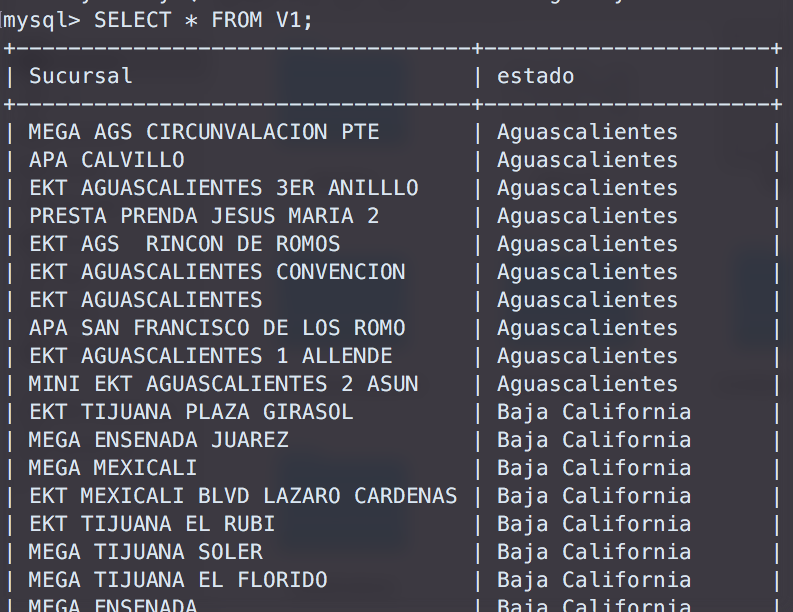
\includegraphics[width=0.35\textwidth]{BD5Reporte1}
            \caption{Nombre de la Sucursal y el estado donde esta}
        \end{figure}

        \begin{figure}[ht!]
            \centering
            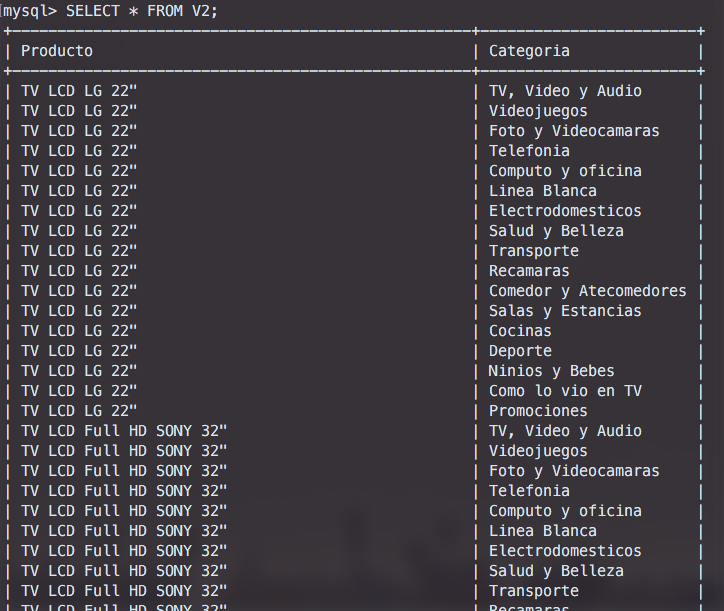
\includegraphics[width=0.35\textwidth]{BD5Reporte2}
            \caption{Nombre del Producto y su Categoria}
        \end{figure}


        \begin{figure}[ht!]
            \centering
            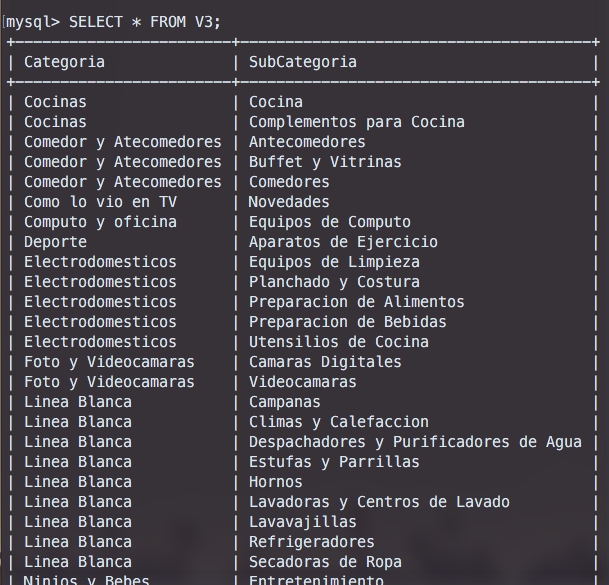
\includegraphics[width=0.35\textwidth]{BD5Reporte3}
            \caption{Nombre de la Categoria y Subcategoria}
        \end{figure}

        \begin{figure}[ht!]
            \centering
            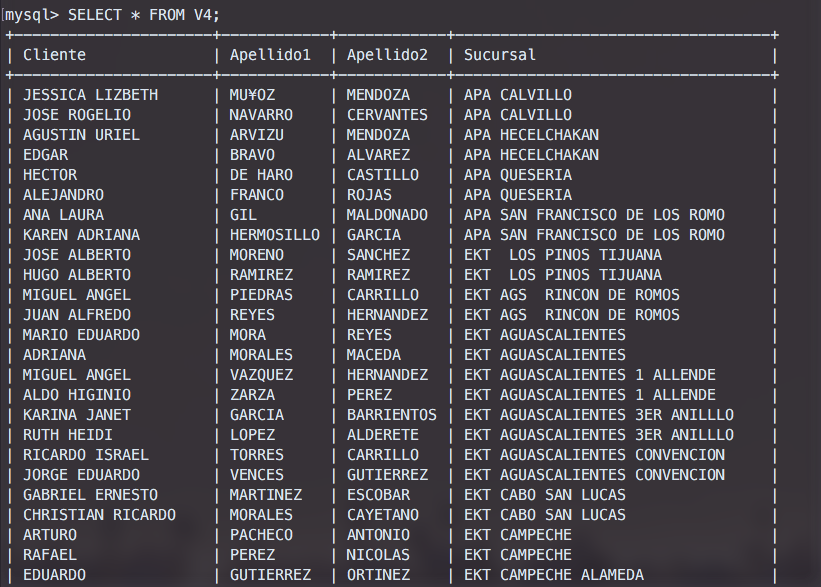
\includegraphics[width=0.35\textwidth]{BD5Reporte4}
            \caption{Nombre del Cliente y Sucursal donde fue dado de alta}
        \end{figure}

        \begin{figure}[ht!]
            \centering
            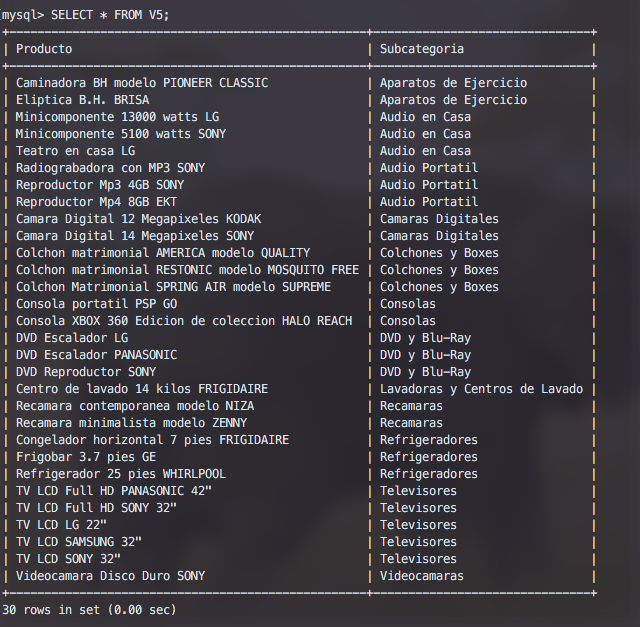
\includegraphics[width=0.35\textwidth]{BD5Reporte5}
            \caption{Nombre del Producto y su Subcategoria}
        \end{figure}

        \begin{figure}[ht!]
            \centering
            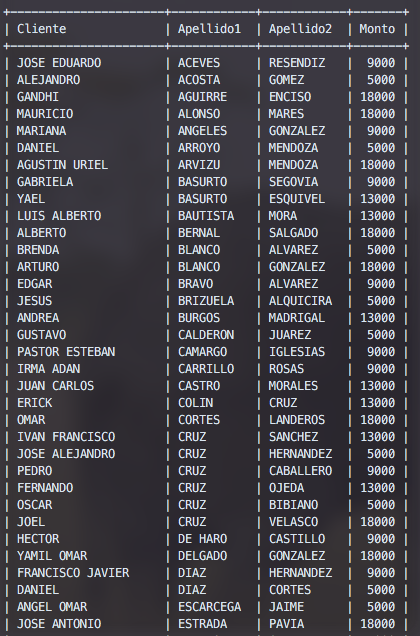
\includegraphics[width=0.45\textwidth]{BD5Reporte6}
            \caption{Nombre del Cliente y monto del Credito}
        \end{figure}

        \begin{figure}[ht!]
            \centering
            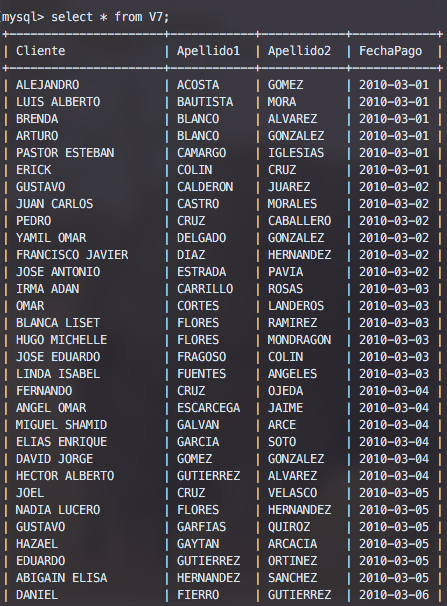
\includegraphics[width=0.45\textwidth]{BD5Reporte7}
            \caption{Nombre del Cliente y fechas de pago}
        \end{figure}


        \begin{figure}[ht!]
            \centering
            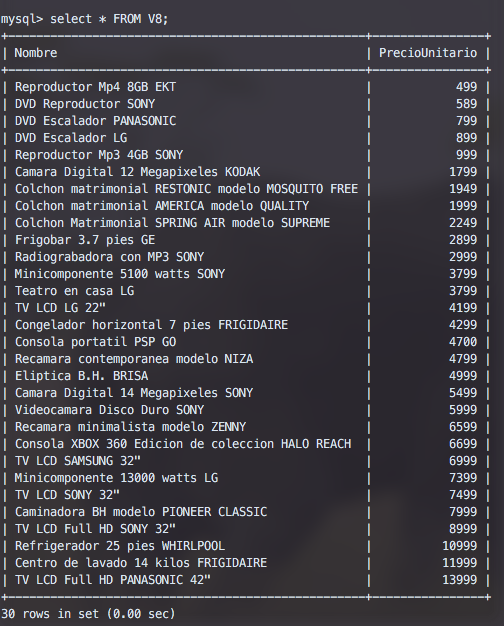
\includegraphics[width=0.45\textwidth]{BD5Reporte8}
            \caption{Nombre del Producto y Precio Unitario}
        \end{figure}

        \begin{figure}[ht!]
            \centering
            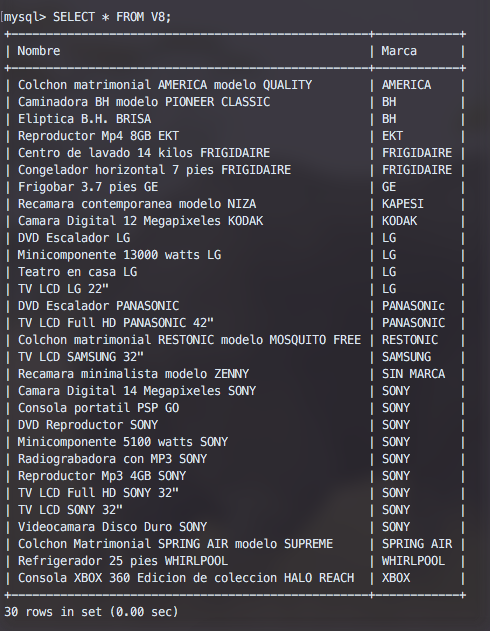
\includegraphics[width=0.45\textwidth]{BD5Reporte9}
            \caption{Nombre del Producto y su Marca}
        \end{figure}

        \begin{figure}[ht!]
            \centering
            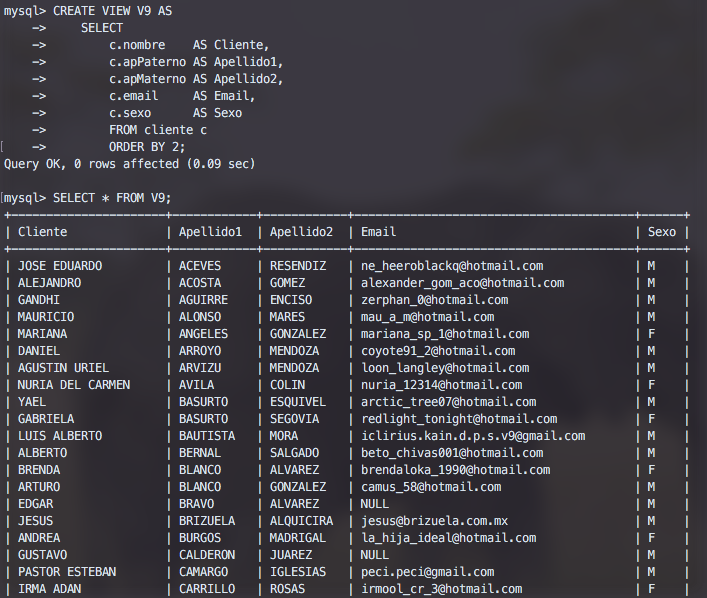
\includegraphics[width=0.45\textwidth]{BD5Reporte10}
            \caption{Nombre del Cliente, Email y su género}
        \end{figure}

        \begin{figure}[ht!]
            \centering
            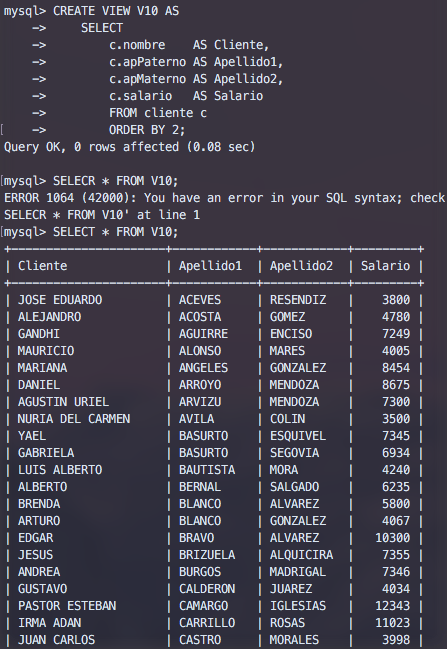
\includegraphics[width=0.45\textwidth]{BD5Reporte11}
            \caption{Nombre del Cliente y su Salario}
        \end{figure}

        \clearpage

        \begin{figure}[ht!]
            \centering
            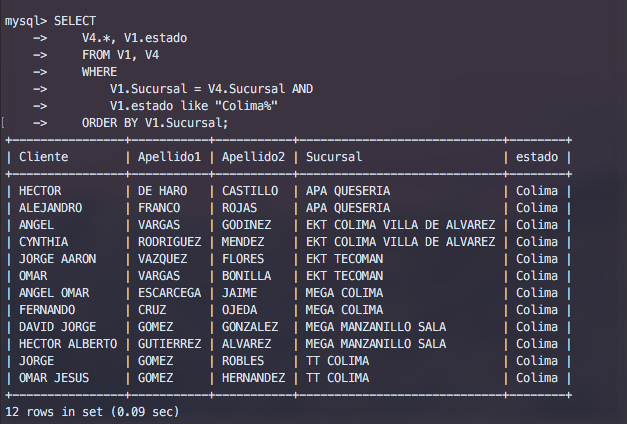
\includegraphics[width=0.45\textwidth]{BD5Reporte2Parte1}
            \caption{Clientes en las sucursales de Colima}
        \end{figure}

        \begin{figure}[ht!]
            \centering
            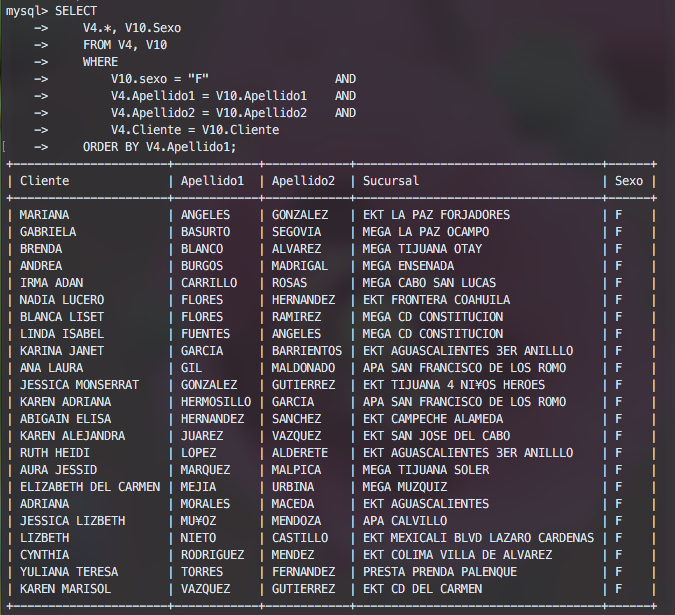
\includegraphics[width=0.45\textwidth]{BD5Reporte2Parte2}
            \caption{Sucursales donde hay mujeres}
        \end{figure}

        \begin{figure}[ht!]
            \centering
            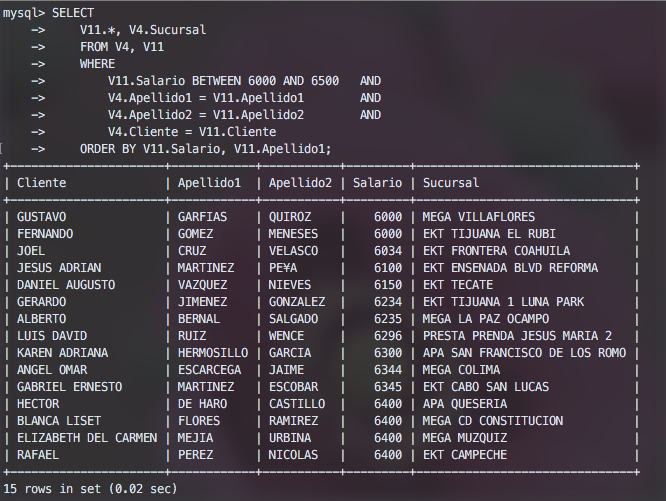
\includegraphics[width=0.45\textwidth]{BD5Reporte2Parte3}
            \caption{Clientes que ganan entre 6k y 6.5k, incluir sucursales}
        \end{figure}


        \begin{figure}[ht!]
            \centering
            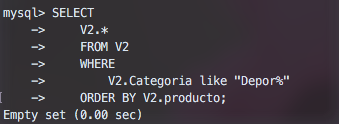
\includegraphics[width=0.45\textwidth]{BD5Reporte2Parte4}
            \caption{Productos de Deporte}
        \end{figure}

        \begin{figure}[ht!]
            \centering
            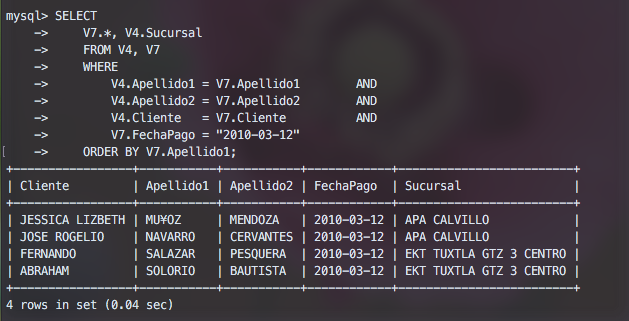
\includegraphics[width=0.45\textwidth]{BD5Reporte2Parte5}
            \caption{Clientes que pagaron en 12 Marzo de 2010, incluir de la Sucursal}
        \end{figure}





% ===============================================================================
% ===================           CONCLUSIONES               ======================
% ===============================================================================
\clearpage
\section{Conclusiones}

    Gracias a esta practica pudimos comprender mucho mejor como es que funcionan las bases de datos
    y lo facil que puede llegar a ser crear vistas, declararlas y como hacer consultas con el.

    Vimos lo poderoso que puede llegar a ser SQL y como podemos modificar nuestros querys usando las 
    views, sus ventajas y lo fácil que hacen crear una consulta que antes era muy compleja



% =====================================================
% ============        BIBLIOGRAPHY   ==================
% =====================================================
\bibliographystyle{plain}
\begin{thebibliography}{9}

    % ============ REFERENCE #1 ========
    \bibitem{Libro} 
        \texttt{Databases, Liberty Hall Chichester 1999}
        Bob Hudson

    \bibitem{Libro2} 
        \texttt{Computer Science Distilled,}


     

\end{thebibliography}




\end{document}

